\documentclass[apj,tighten]{emulateapj}
\makeatletter
\parskip .7em         % sets inter para spacing at .7ems
\textheight 10.0in     % sets textheight
\textwidth 7.5 in      % sets textwidth
\voffset -1in       %
\hoffset -0.50in       % sets vert. and horiz offsets
 \journalinfo{ }
 \submitted{}
\usepackage{wasysym, multirow, soul, graphicx}
\usepackage{hyperref}
\usepackage[usenames,dvipsnames]{color}
\usepackage{gensymb}
\def\Rsat{$\mathrm{R}_{\mathrm{\saturn}}$} 
\def\um{\mathrm{$\mu$m}}
 
\shorttitle{Titan's NSA at Equinox}
\shortauthors{Vashist \emph{et al.}}
\bibpunct[, ]{(}{)}{;}{a}{,}{,}

\begin{document}
\title{Titan's North-South Asymmetry at visible wavelength over the Cassini Mission}

% All Authors
\author{Aadvik Vashist\altaffilmark{1,3}, Michael F. Heslar\altaffilmark{1}, Jason W. Barnes\altaffilmark{1}, Corbin Hennen\altaffilmark{1},
Ralph D. Lorenz\altaffilmark{2}}
\altaffiltext{1}{Department of Physics; University of Idaho; Moscow, ID 83844}
\altaffiltext{2}{Johns Hopkins University Applied Physics Laboratory; Laurel, MD 20723}
\altaffiltext{3}{River Hill High School; Clarksville, MD; 21029}

%Abstract
\begin{abstract}
We document the evolution of the North-South Asymmetry (NSA) of Titan's haze albedo during the \textit{Cassini} mission between 2004 and 2017.
We analyze co-added cube images taken at 96 distinct wavelengths between 0.35-1.05 $\mu$m by the \textit{Cassini} Visual and Infrared Mapping Spectrometer (VIMS-V) instrument from 14 Titan flybys.
Over half of a Titan year, we observe a near-complete transition in the NSA boundary latitude across the geographic equator from the southern to the northern hemisphere, including a 3-year fading of the boundary for several years after the equinox.
The fading transition of the NSA matches previous observations of a reversal of the NSA in Hubble images of Titan before the winter solstice between 1997-2000. A comparison of NSA images taken at similar times but different phase angles shows the NSA boundary is detectable, albeit with less contrast, at moderately high phase angles ($\sim$90\degree). Analysis of the NSA boundary in T61 and T67 VIMS images further supports a small tilt between the super-rotating atmosphere and the solid body of Titan, as  suggested in a previous analysis of 0.890 $\mu$m images from the \textit{Cassini} Imaging Science Subsystem (ISS). 
\end{abstract}
\keywords{Titan, Upper atmosphere, Seasonal phenomena}

\section{INTRODUCTION}

Saturn's moon Titan exhibits many properties not found in other satellites. As first observed by Voyager 1 \citep{smith1981encounter}, Titan's ubiquitous atmospheric haze prevents optical imaging of the surface (\cite{richardson2004113}; \autoref{figure:nsa_vis}).
The haze distribution varies as a function of latitude \citep{Sromovsky1981}, altitude \citep{smith1982new,tomasko2005rain}, and time \citep{lorenz1997titan,west2011evolution}. 
Titan's haze also shows albedo differences between its northern and southern hemispheres that shift near the equator.
\autoref{figure:nsa_2bands} shows how these differences are also dependent on wavelength.
As the seasons progress, atmospheric circulation changes the global haze distribution, culminating in a seasonal reversal every 14 years (\cite{brown2009titan};\autoref{figure:ifAcrossFlybys}, \autoref{figure:flux}).
The reversal presents as an albedo dichotomy in the otherwise featureless atmosphere.
The existence of the asymmetry also results in a  distinct boundary that separates the north and south hemispheres.


The Voyager 1 flyby highlighted the existence of a North-South Asymmetry (NSA) between the two hemispheres \citep{smith1981encounter}.
Previous discoveries also found a tilt of the boundary line relative to the solid-body equator of Titan \citep{Roman2009}.
The boundary, as reported by \citep{Sromovsky1981} with Voyager 1 data, was located at roughly 5.5\degree{}S.
More recent discoveries show a seasonal reversal in the latitude of the asymmetry across the equator. 


Movement of the NSA boundary reveals important details of the global atmospheric properties and circulation patterns of Titan \citep{hirtzig2006monitoring}.
Titan disk observations from flyby missions and professional telescopes provide sporadic temporal and wavelength coverage of the NSA, leading to incomplete records on haze circulation with large errors \citep{lorenz2001titan,lorenz2004seasonal}.
In addition, previous studies often use special case methodologies, where results are tied to their data-sets to calculate and subsequently compare those previous NSA boundary latitudes \citep{Roman2009}.
These methodologies can be modified to fit a wider range of data \autoref{figure:flowchart}.


More recent studies have the temporal coverage to study detailed aspects for a substantial portion of the NSA cycle with individual data sets.
\cite{karkoschka2022titan} modeled the NSA reversal at different altitudes with HST Space Telescope Imaging Spectrograph image cubes.
\cite{kutsop2022titan} completed an analysis of circumglobal haze bands in a variety of Cassini imagery data sets. 


In this paper, we document on the seasonal changes in Titan's lower atmospheric haze near the equator using the \textit{Cassini} observations of visible wavelengths for purposes of comparison with previous studies.
The observation of seasonal haze changes through visible wavelengths allows us to extend the time baseline of previous observations and to coherently track one seasonal cycle with a single uniform dataset.
The \textit{Cassini} Visual and Infrared Mapping Spectrometer (VIMS) collected spectral maps at 96 visible and near-infrared wavelengths between 0.35-1.05 $\mu$m, which predominantly sampled the stratosphere ($\sim$70-120 km).

Section 2 elaborates on the selection criteria for our dataset (\autoref{table:data}) and describes how we modify the main NSA image analysis algorithm from \citep{Roman2009} with considerations for the VIMS data characteristics.
In section 3, We determine the latitude of the asymmetry at 76 of the 96 distinct wavelengths, excluding atmospheric windows where the surface is visible and precluding haze measurements (\cite{vixie2012mapping}, \autoref{figure:hc_bands4}).
Each distinct wavelength accesses a different altitude because of the varying atmospheric opacity.
In section 4, we locate the latitude of the NSA on 13 distinct flybys.
We also determine the albedo contrast between the northern and southern hemispheres with regard to wavelength to calculate the boundary latitude, north-south flux ratios, and tilt angles of the asymmetry (\autoref{figure:tiltT61}). Additionally, we highlight the difference between low and high-phase angle I/F profiles(\autoref{figure:lo_vs_hi_phase3}), and contextualize our results within the Titanian orbit (\autoref{figure:nsadisappears}, \autoref{figure:nsaTime})
Finally, in section 5, we compare our results to the existing archive of NSA boundary observations and discuss the implications of these findings on the atmospheric conditions of Titan.


\begin{figure}[!htbp]
\includegraphics[width=\columnwidth]{figures/nsa_vis.png} 
\caption{\footnotesize A T62 image of VIMS cube CM$\_$1634082284$\_$1 taken on 12 October 2009 shows a typical low-phase angle view of Titan with the North-South Asymmetry (NSA) at visible wavelengths from the VIMS instrument (VIMS-V).
The colors are an approximation of true color using the VIMS-V channels.
The overall orange color comes from haze scattering and atmospheric absorption (primarily methane).
North is upwards in the image.
\label{figure:nsa_vis}}
\end{figure}


\begin{figure}[!htbp]
\includegraphics[width=\columnwidth]{figures/nsa_2wvlns.png}
\caption{\footnotesize Titan’s NSA is evident in two individual band images from the same VIMS cube in \autoref{figure:nsa_vis} (CM$\_$1634082284$\_$1).
In the left cube, the southern hemisphere appears brighter at blue wavelengths.
In contrast, the NSA reverses in the right image within a methane absorption band at 0.886 $\mu$m. Vertical striping artifacts are present in the images.
\label{figure:nsa_2bands}}
\end{figure}


\section{OBSERVATIONS and METHODS}

As shown in \autoref{table:data}, we analyze Cassini VIMS observations from 12 targeted flybys from 2004-2015 and 2 non-targeted flybys from 2017 of Titan.
Each flyby observed Titan from $ 0.356\mu$m to 1.046 $\mu$m in 96 distinct wavelength channels to sample from the Southern Summer to Northern Summer transition \citep{brown2004cassini}. 
We selected these particular flybys based on boundary visibility, sufficient time cadence, and time frame so as to obtain measurements spaced out over the entire period of \textit{Cassini} observations.
For a majority of the flybys, the spatial sampling per pixel is $\sim$45 km or 1\degree{} of latitude. 


For the NSA, one hemisphere appears brighter and the other dimmer, with a semi-distinct line near the tropics (i.e., low latitudes) dividing the two.
Which hemisphere is which depends on the season and the observed wavelength that samples at different altitudes as shown in \autoref{figure:nsa_2bands}.
\cite{lorenz1997titan} attributes the reversal to the separately varying single-scattering albedo of the haze and gas as a function of wavelength. 
At short visible wavelengths (\autoref{figure:nsa_2bands}, left), the haze has a low albedo, but the gas itself is relatively bright due to Rayleigh scattering. Thus, more haze leads to a darker hemisphere at short wavelengths. 
At near-infrared wavelengths close to the visible (\autoref{figure:nsa_2bands}, right), however, the haze single-scattering albedo is high, and methane starts to absorb, making the gas dim. 
So higher haze concentrations make a hemisphere brighter at long wavelengths. 


The present work makes use of a collection of \textit{Cassini} VIMS image cubes from the mission.
The images have a variety of spatial samplings (owing to different spacecraft distances).
We also chose these particular flybys as ones where a majority or all of Titan's disk is observed. 


\autoref{figure:flowchart} outlines our VIMS image processing algorithm.
An issue found in the VIMS data is the vertical striping noise in the original images.
We could not directly correct the striping noise because the data used to subtract the background on board Cassini was not transmitted back to Earth \citep{brown2004cassini}.
To mitigate the striping issues, we increased the signal-to-noise ratio by co-adding images, and then mapping the final co-added image onto a cylindrical projection \citep{vixie2012mapping}.
The spatial sampling of the cylindrical images is $\sim$45 km or 1\degree{} of latitude.
Note that the vertical striping appears as superimposed stripes across cylindrical projections.
Additionally, these projections do not include limb pixels and thus minimize limb-darkening effects.
Images at 96 distinct wavelengths, also known as bands, were created for each flyby. 


After we generate a final set of images, we adapt the methods from \cite{Roman2009} to determine the latitude of the NSA boundary.
We shift the images by 6°N and 6°S, and then subtract to create a brightness contrast of each image, which highlights the presence of an asymmetry \citep{Roman2009}.
These maps were then sequentially analyzed along each longitude using a sixth-order polynomial fit to smooth out signal variations.
We found the locations of critical points using the derivative function of the fit; extraneous values, such as imaginary solutions and numbers outside of the latitude range, were removed to leave only the latitude location of the NSA at each longitude column.
Our algorithm then finds the latitude value of the NSA transition for all the columns within each projection and then averages them to determine the location of the NSA for each band in the flyby.
Since each column has a varied value for the NSA, we applied a moving average to the data to flatten irregularities in column brightness data.
Using the latitude value found in each image, we apply a simple average of the brightness 30°N and 30°S of the NSA transition to determine the North/South Flux Ratio.
We derive I/F values using average visible latitude, where each latitude is an average of all visible longitudinal brightness values. 


We can attribute inaccuracies in all results to sampling area, surface wavelengths, and/or a deterioration in image quality and accuracy over the course of the Cassini mission. We can find uncertainties in our uncertainty in our image processing algorithm through the standard deviation of the derived latitude value of every image. \textbf{NEEED TO PUT STUFF HERE}


\begin{figure*}[!hb]
\includegraphics[width=\textwidth]{figures/NS Flowchart.png}
\caption{\footnotesize Here we present a flowchart of the image processing procedures to obtain the NSA boundary latitude and the NS flux ratio from an individual VIMS cube image.
\label{figure:flowchart}}
\end{figure*}


\section{NORTH-SOUTH ASYMMETRY} \label{nsa}

\begin{figure*}[h]
\centering
\includegraphics[height = 24cm, keepaspectratio]{figures/IF.png}
\caption{\footnotesize Meridional disk brightness (I/F) profiles across Titan from select flybys over a Titan half-year. The top plot shows the profile at 0.550 $\mu$m, the middle for 0.695 $\mu$m, and the right for 1.003 $\mu$m. The profile did not exhibit much change between 2004 and 2007 (Ta-T31). With the onset of the vernal equinox in T61, the meridional profile developed dramatic changes and underwent a complete flip by 2017 (278TI).
\label{figure:ifAcrossFlybys}}
\end{figure*}


\begin{figure*}[tbhp]
\includegraphics[width=\textwidth]{figures/Flux.png}
\caption{\footnotesize NS flux ratio spectra (average ratio of I/Fs 30\degree{}
above and below the NSA boundary latitude) from select flybys over a Titan half-year.
Note that wavelengths where methane absorbs (e.g., 0.89 $\mu$m)
tend to show an inverted NS flux ratio relative to methane windows (e.g., 0.93 $\mu$m).
Ta and T8 spectra show distinct features, while T114 and 278TI spectra show those same features with a flipped concavity.
The other spectra from T31 to T108 that were recorded closer to the vernal equinox show subdued or nonexistent features, indicating a more uniform meridional haze profile for Titan.
\label{figure:flux}}
\end{figure*}


\subsection{Meridional Brightness Profiles} 

\autoref{figure:ifAcrossFlybys} displays various meridional brightness profiles from specific flybys at two wavelengths: one near-infrared and one visible.
At certain wavelengths, the location of the boundary generally corresponds with either maxima or minima of the profiles, depending on the season.
The values of each profile are averaged over longitude to minimize noise from striping and various other artifacts.

Flybys from the Prime mission (2004-2008) in Southern Summer have a single relative maximum that increases in latitude as time progresses, whereas later flybys show greater variance.
The movement of the relative extrema also serves to visualize the changes in the North-South flux ratio.
We note that limited spatial coverage in the VIMS images of the non-targeted flybys (278TI, 283TI) causes the early cutoff in their NS flux ratio profiles just below the equator in \autoref{figure:ifAcrossFlybys}. 


\subsection{NS Flux Ratio Spectra}
\autoref{figure:flux} displays the contrast ratio as a function of the regions 30\degree{} north and south of the NS boundary in three panels for northern winter, equinox, and northern summer.
The total observed time equates to about half a titan year.
The top panel in \autoref{figure:flux} shows that the region south of the NS boundary is brighter across all wavelengths except in methane bands, like 0.89 $\mu$m.
At the equinox, the North-South flux ratio increases until the profile have NS flux ratio values greater than 1, indicating a meridional movement of the stratospheric haze layers.
The flat T108 NS flux ratio profile during northern summer indicates that the NSA has disappeared at all wavelengths.
Then in 2017, we observe a new set of inverted profiles with NS flux ratios over 1 at visible wavelengths of 0.4-0.75 $\mu$m and below 1 at infrared wavelengths of 0.8-1.05 $\mu$m.
The profile inversion suggests the formation of a new NS boundary above the equator. 

Outlier fluctuations in the NS flux ratio can be attributed to a wavelength-dependent haze single-scattering albedo and atmospheric gaseous absorption.
We observe a gradual increase in the NS flux ratio as time progress through the flybys with a minimum value of 0.773 at 0.51 $\mu$m in the Ta flyby, 1.034 at 0.41 $\mu$m for T67, and 1.25 at 1.03 $\mu$m for T108.
As for averages, Ta, T67, and T108 exhibit an average flux ratio of 0.922, 1.17, and 1.29, respectively.

\subsection{Implications for Global Circulation}
The evolution of the meridional haze brightness profiles over the Cassini mission trace atmospheric circulation at different altitudes in the stratosphere.
Insolation, the quantity of solar radiation received by a certain area, drives a Hadley circulation of the upper atmosphere with upwelling at the summer pole and subsidence at the winter pole \citep{tokano2007near,lebonnois2014general}, driving up haze concentration in the winter hemisphere.
The observed reversal in the NS meridional brightness profile before and after the equinox records a clear trend of global Hadley haze circulation driven by seasonal changes in insolation.
The NS flux ratio spectra show a similar reversal (across the NS flux ratio value of 1 or the red dashed line in \autoref{figure:flux}) in the methane absorption band profiles over the seasons at visible and infrared wavelengths sampling at altitudes between 60-250 km \cite{robinson2014titan}.
The combination of the meridional profile and NS flux ratio spectra observations over a Titan half-year further support the idea of a positive feedback loop between the global atmospheric circulation patterns and haze production \cite{rannou2002wind}. 
Our results on the contrasting brightness profiles match well with other recent works analyzing the NSA brightness differences with spectral models \cite{kutsop2022titan} and modeling haze concentrations associated with the NSA using Principal Component Analysis \citep{karkoschka2022titan}.


\section{NORTH-SOUTH BOUNDARY}

\subsection{Boundary Latitude}


The straight-line interhemispheric boundary was the most prominent feature in the first high quality spatially-resolved images of Titan, those by the Voyager 1 spacecraft in 1980.
The initial examination of those images suggested that the boundary was within 5\degree{} of the equator near the northern spring equinox \citep{smith1981encounter}.
The location of the boundary as seen by Voyager 2 nearly a year later was essentially identical: \cite{squyres1984voyager} determined the latitude of the boundary with some precision in both data-sets to be 5.5\degree{}$\pm$1\degree{S}.
\cite{flasar1981titan} observed a strong super-rotation of the Titan atmosphere at all latitudes through temperature variations.
The slow rotation of Titan makes its super-rotating atmosphere more prominent. 

The haze changes documented in our study suggest that the stratosphere exhibits a seasonal evolution of Hadley circulation patterns.
There were no resolved observations of Titan between Voyager 2 in 1981 and 1990, when the new Hubble telescope imaged Titan.
However, the deconvolution of Hubble images fit with models \citep{caldwell1992titan} that suggested that the boundary was located at 32\degree{}N$\pm$10\degree{}.

\cite{lorenz1997titan} reported that the best fit for post-repair HST images acquired in 1994 and 1995 suggested that the boundary was between 10 and 20\degree{N}.
Further HST images in 1997 and 2000 were examined by \cite{lorenz2004seasonal} - and although the appearance in each case is not inconsistent with a near-equatorial boundary, the contrast is both weak and takes the form of a ramp rather than a step, so it was difficult to define a precise boundary latitude.
During the northern winter from 2002-2003, an inspection of N-S profiles of 0.435 $\mu$m HST images \cite{lorenz2006seasonal} also showed a ramp in albedo ratio (the sharpness of the albedo boundary is in part reduced owing to the telescope point spread function), but the contrast was then large enough (in a sense opposite from that in the mid-1990s) such that mid-point of the ramp could define an approximate boundary. 
The December 2002 image ramp spanned 40\degree{}S to 10\degree{}S, and thus the midpoint is 20\degree{}S to 22\degree{}S; the 2003 image ramp is a little better defined and spanned 45\degree{}S to 0\degree{}.
The difference in position between 2002 and 2003 did not appear to be significant (although the contrast between hemispheres did increase noticeably).
Examination of the 2002 images at 0.502 $\mu$m and 0.892 $\mu$m suggests a similar contrast boundary latitude within 5 degrees at those wavelengths.
From the mission, \cite{Roman2009} analyzed \textit{Cassini} ISS images taken from 2004 to 2007 to pin down the clear NSA boundary to $\sim$8\degree{S} within an error margin of 2\degree{}.

Now, we show observations from VIMS cube images taken from flybys acquired over the entire \textit{Cassini} mission in \autoref{figure:hc_bands4}.
We adopt a stretch that enhances the visibility of the high-contrasting band for \autoref{figure:hc_bands4} which also tends to accentuate noise and instrument artifacts.
Between the Ta and T92 flybys, we observe the high-contrasting band South of the equator (red dashed line in \autoref{figure:hc_bands4}). 

After T92, the high-contrasting band is not visible in all targeted flyby images (e.g., T108), and instead, multiple bands appear at random locations far from the equator. 
The extra bands are consistent with observations of secondary bands appearing during the northern summer \citep{kutsop2022titan}, but are not the focus of this publication. The NSA boundary latitudes stay at fairly constant values of 8-11\degree{S}.
We only witness the return of the high-contrasting band in two non-targeted flybys 278TI and 283TI, images of Titan in mid-2017, which owing to spacecraft observation geometry only include half-disk observations just below the equator.
However, the high-contrasting band in the 2017 images indicate that the NSA boundary flipped across the equator.
The new NSA boundary latitude was approximately 10\degree{N} within an error margin of 4\degree{}. 



\subsection{Boundary Tilt}
Looking further at the high-contrasting bands in \autoref{figure:hc_bands4}, many of the bands appear to be slanted or tilted with respect to the geographic equator. 
The tilt angle is positive for  high-contrasting bands oriented above the geographic equator. 
\cite{Roman2009} made a similar observation of a tilt in the NSA during the early flybys from 2004 to 2007.
Visually speaking, the tilts of the high-contrasting bands in our VIMS images for select flybys (Ta, T31, T62) do not appear linear across all longitudes.
That is, they remain horizontal on the left side of the band until starting a gradual upward tilt on the right side. Nonetheless, we chose to use the higher-quality VIMS observations from T67 to deduce tilt measurements with a least-squares linear regression, shown in \autoref{figure:tiltT61}. 
Overall, we find further evidence for a small, detectable tilt of the NSA boundary, despite the lower spatial sampling of the VIMS cube images. 
Similar measures of tilt angle between 2° and 6° were found in an analysis of circumpolar bands in VIMS images \citep{kutsop2022titan}.

Consequently, we find rough estimates for the tilt angle ranging from 1-2\degree{}, as opposed to the 4\degree{} of \cite{Roman2009}. We note that the tilt angle is only one factor influencing the geometry of the NSA boundary in Titan images.
Other factors include an azimuthal offset from the subsolar longitude \citep{Roman2009}.
The origin of the tilt may arise from an offset between the atmospheric and geographic (solid body) poles \citep{Roman2009}. 
It is not obvious that the obliquity of 4\degree{} observed by \cite{achterberg2008titan} in thermal data and by \cite{Roman2009} in 0.889 $\mu$m images should have been constant throughout the seasonal cycle.
Although the tilt angle appears to have remained roughly fixed over 2004-2007 \citep{Roman2009}, this was also fixed from 2004-2017 although the boundary (37\degree{}) does migrate over the course of a year.


\subsection{Low vs. High Phase}


A comparison of NSA images (0.886 $\mu$m) at a low and high phase (88\degree{}) angle is shown in \autoref{figure:lo_vs_hi_phase3}.
The images were taken only 9 months apart for a minimally-biased comparison.
We observe that the NSA boundary is still detectable at a high phase angle, albeit at lower contrast. 
For blue and green wavelengths, the profiles are fairly well aligned with each other in gradient and brightness in \autoref{figure:lo_vs_hi_phase3}c.
For red wavelengths, the meridional profiles show a noticeable difference between the two phase angles.
The high phase profiles show a more gradual gradient and more southerly inflection point from 60\degree{S} to 30\degree{N} relative to the low phase profiles.
For the near-infrared wavelengths, the low and high phase profiles are nearly identical. 
These NSA observations at different phases demonstrate a strong influence of the single-scattering albedo and optical depth on the NSA brightness profile, which varies with wavelength particularly within the methane windows.
Viewing the NSA at a higher phase angle subdues but does not erase the contrast of the boundary. 

\subsection{Seasonal Trends}

We show the seasonal evolution in the hemispheric profile of the NSA using near-infrared colors in \autoref{figure:nsadisappears}.
Purple shows the darker hemisphere, while violet and white shows the brighter hemisphere with a higher haze concentration (refer to \autoref{nsa} for more detail). 
The contrast between the Northern and Southern hemispheres of the boundary is visible when the boundary is located away from the solid-body %rotational
equator (red dashed line in \autoref{figure:nsadisappears}) during 2004-2013 and 2017 but not when the boundary transitions during 2014-2016.  
The boundary transitions between the north and south also experience a decrease in contrast as the boundary approaches the equator.
Eventually, the brightness contrast between the north and south of the boundary fades away, which marks the start of the transitional period in 2014. 

In the T101 and T114 images from \autoref{figure:nsadisappears}, the disk shows a uniform white color that indicates the fading of the hemispheric dichotomy.
The re-emergence of the dichotomy North of the equator does not happen until the latest non-targeted flybys (278TI and 283TI) are noted by the flip in the respective colors of each hemisphere.
The VIMS cube images from non-targeted Titan flybys have poor global coverage and inconsistent striping error that limits the number of usable VIMS cubes.

In our analysis, we document the migration of the NSA boundary during the Cassini solstice mission and prior telescope observations in \autoref{figure:nsaTime}.
From 2004 to 2010, the boundary remains at a steady 11.8\degree{}S, but then experiences a sudden change from 2012 to 2014, where the boundary moves from 9.8\degree{}S to 5.0\degree{}S.
The motion of the NSA boundary in this 2-year period is also similar to the previous post-equinox period from 1995 to 1997 \citep{lorenz1999seasonal}.
Over the next 4 years, the N/S Ratio not only reverses but the NSA boundary is observed to be at $\sim$10\degree{}N, corresponding to a change of $\sim$15\degree{} ($\sim$673 km).
A similar report of the NSA reversal in an analysis of Hubble Space Telescope Imaging Spectrograph taken from 1998-2004 and 2017-2019 \citep{karkoschka2016seasonal,karkoschka2022titan} corroborates with our finding.

Our new observations resemble the report of a rapid change in the NSA at 0.889 $\mu$m between 1997 and 2000 \citep{lorenz2001titan} and confirm the initiation of the NSA reversal across the equator occurs 2-3 years after the equinox.
The VIMS observations constrain the 5-year transition period into behaviors that are nearly identical to previous NSA observations after the equinox (\cite{Sromovsky1981}, \cite{lorenz1999seasonal}, \cite{lorenz2001titan}).
\textbf{TALK TO JASON ABOUT THIS. THE BEHAVIORS ARE EXPLAINED IN THE NEXT SENTENCE}A few years after the equinox, the NSA boundary begins moving towards the equator at a rate of a few degrees of latitude per year for $\sim$2 years.
Afterward, the NSA boundary vanishes during a turbulent period of global Hadley circulation until the haze particles settle out of the upper atmosphere. 

The evolution of the NSA boundary over a Titan year can be broken up into two distinct periods of change.
One period includes a constant extrema latitude for several years until the equinox, followed by the second period of rapid linear change, and the distinct NSA fades away until the boundary reappears on the other side of the equator.
Seasonal variations in the global atmospheric circulation may vary the NSA latitude for each extremum of the NSA cycle. 


\begin{figure*}[tbhp]
\centering
\includegraphics[width=0.75\textwidth]{figures/hc_bands6.png}
\caption{\footnotesize Cylindrical projection maps of the high contrasting band for every flyby with a faint demarcation of the equator in red.
The dark band is visible in most flyby images.
We note two distinct bands far from the equator in the T108 image, which hints at the lack of an NSA boundary.
\label{figure:hc_bands4}}
\end{figure*}

\begin{figure*}[tbhp]
\includegraphics[width=\textwidth]{figures/TiltT67.png}
\caption{\footnotesize The top and bottom panels show T67 VIMS cube images at 0.886 and 1.003 $\mu$m, respectively, these maps show a visible tilt in the NSA boundary. The red line tracks individual measurements of the NSA boundary latitude for image columns where the NSA is evident. The blue line shows a linear regression model fit for those NSA boundary latitudes to determine a tilt angle for the NSA boundary. The linear fit indicates that at 0.886 $\mu$m, the NSA boundary is located 12°S ± 3° with an angle of -0.81° \textbf{GET UNCERTAINTY FOR THE ANGLES}. At 1.003 $\mu$m, the NSA Boundary is at 12°S ± 0° with an angle of -0.55° \textbf{GET UNCERTAINTY FOR THE ANGLES}.
\label{figure:tiltT61}}
\end{figure*}

\begin{figure*}[tbhp]
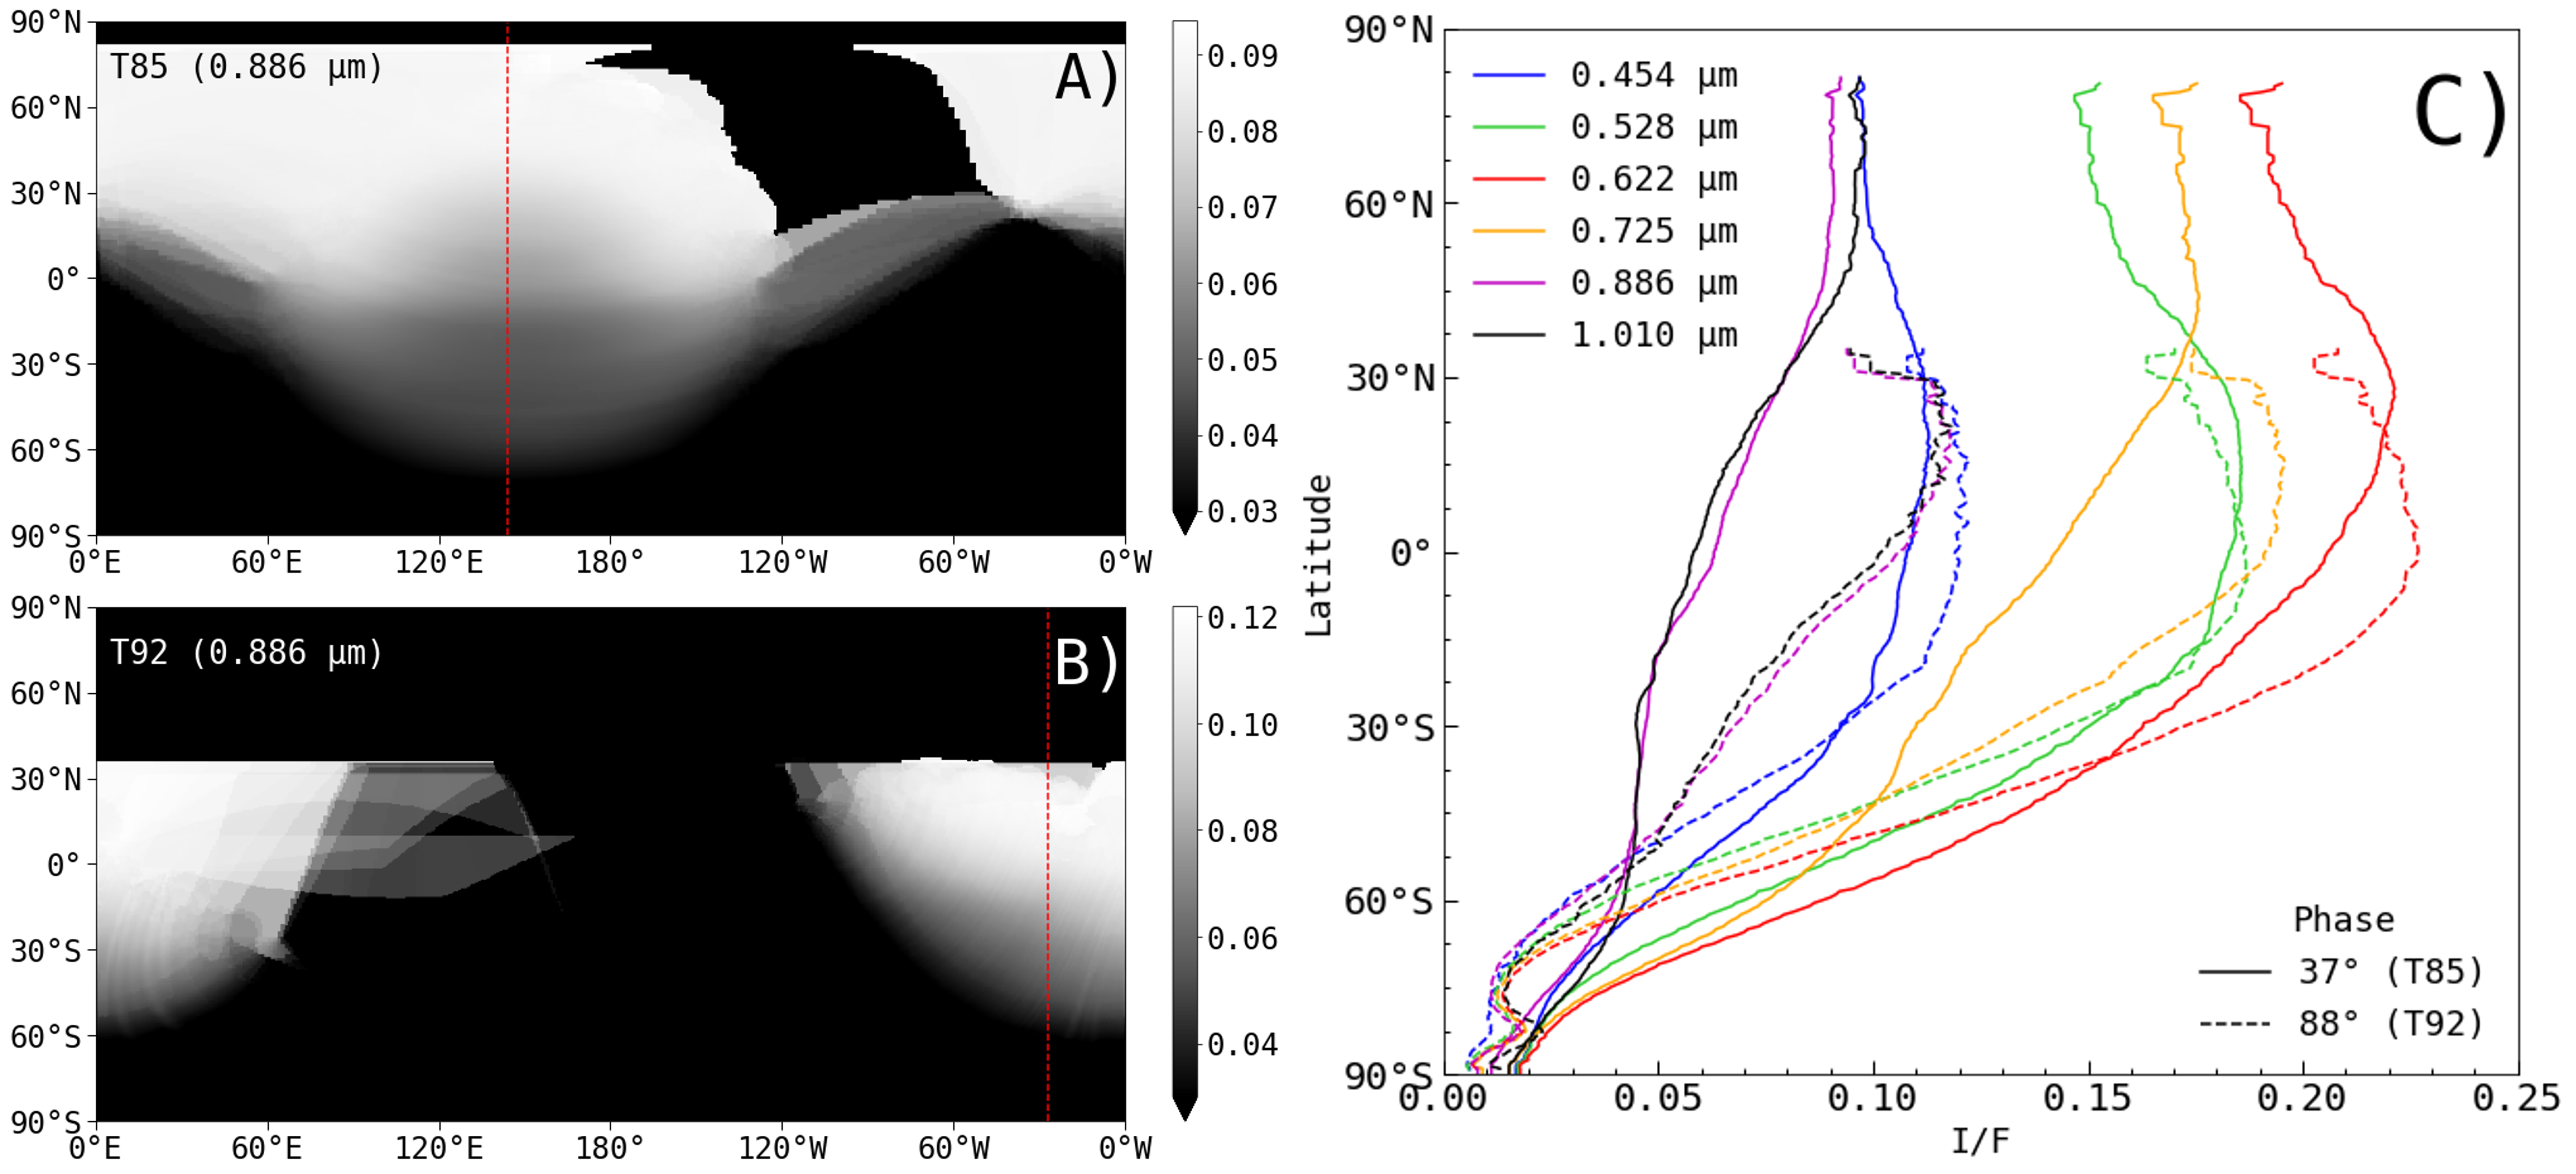
\includegraphics[width=\textwidth]{figures/lo_vs_hi_phase4.png}
\caption{\footnotesize Individual VIMS cube images at 0.886 $\mu$m taken within one year of each other at a low (37\degree{}) and high (88\degree{}) phase angle, respectively. The right plot (C) shows a comparison of the meridional profiles for the two-phase angles in several methane windows. At visible wavelengths, the low-phase profiles show steeper gradients; meanwhile, the near-infrared profiles have no obvious differences. The red dashed lines in (A) and (B) indicate the longitude of the meridional profiles from each image.
\label{figure:lo_vs_hi_phase3}}
\end{figure*}

\begin{figure*}[tbhp]
\centering
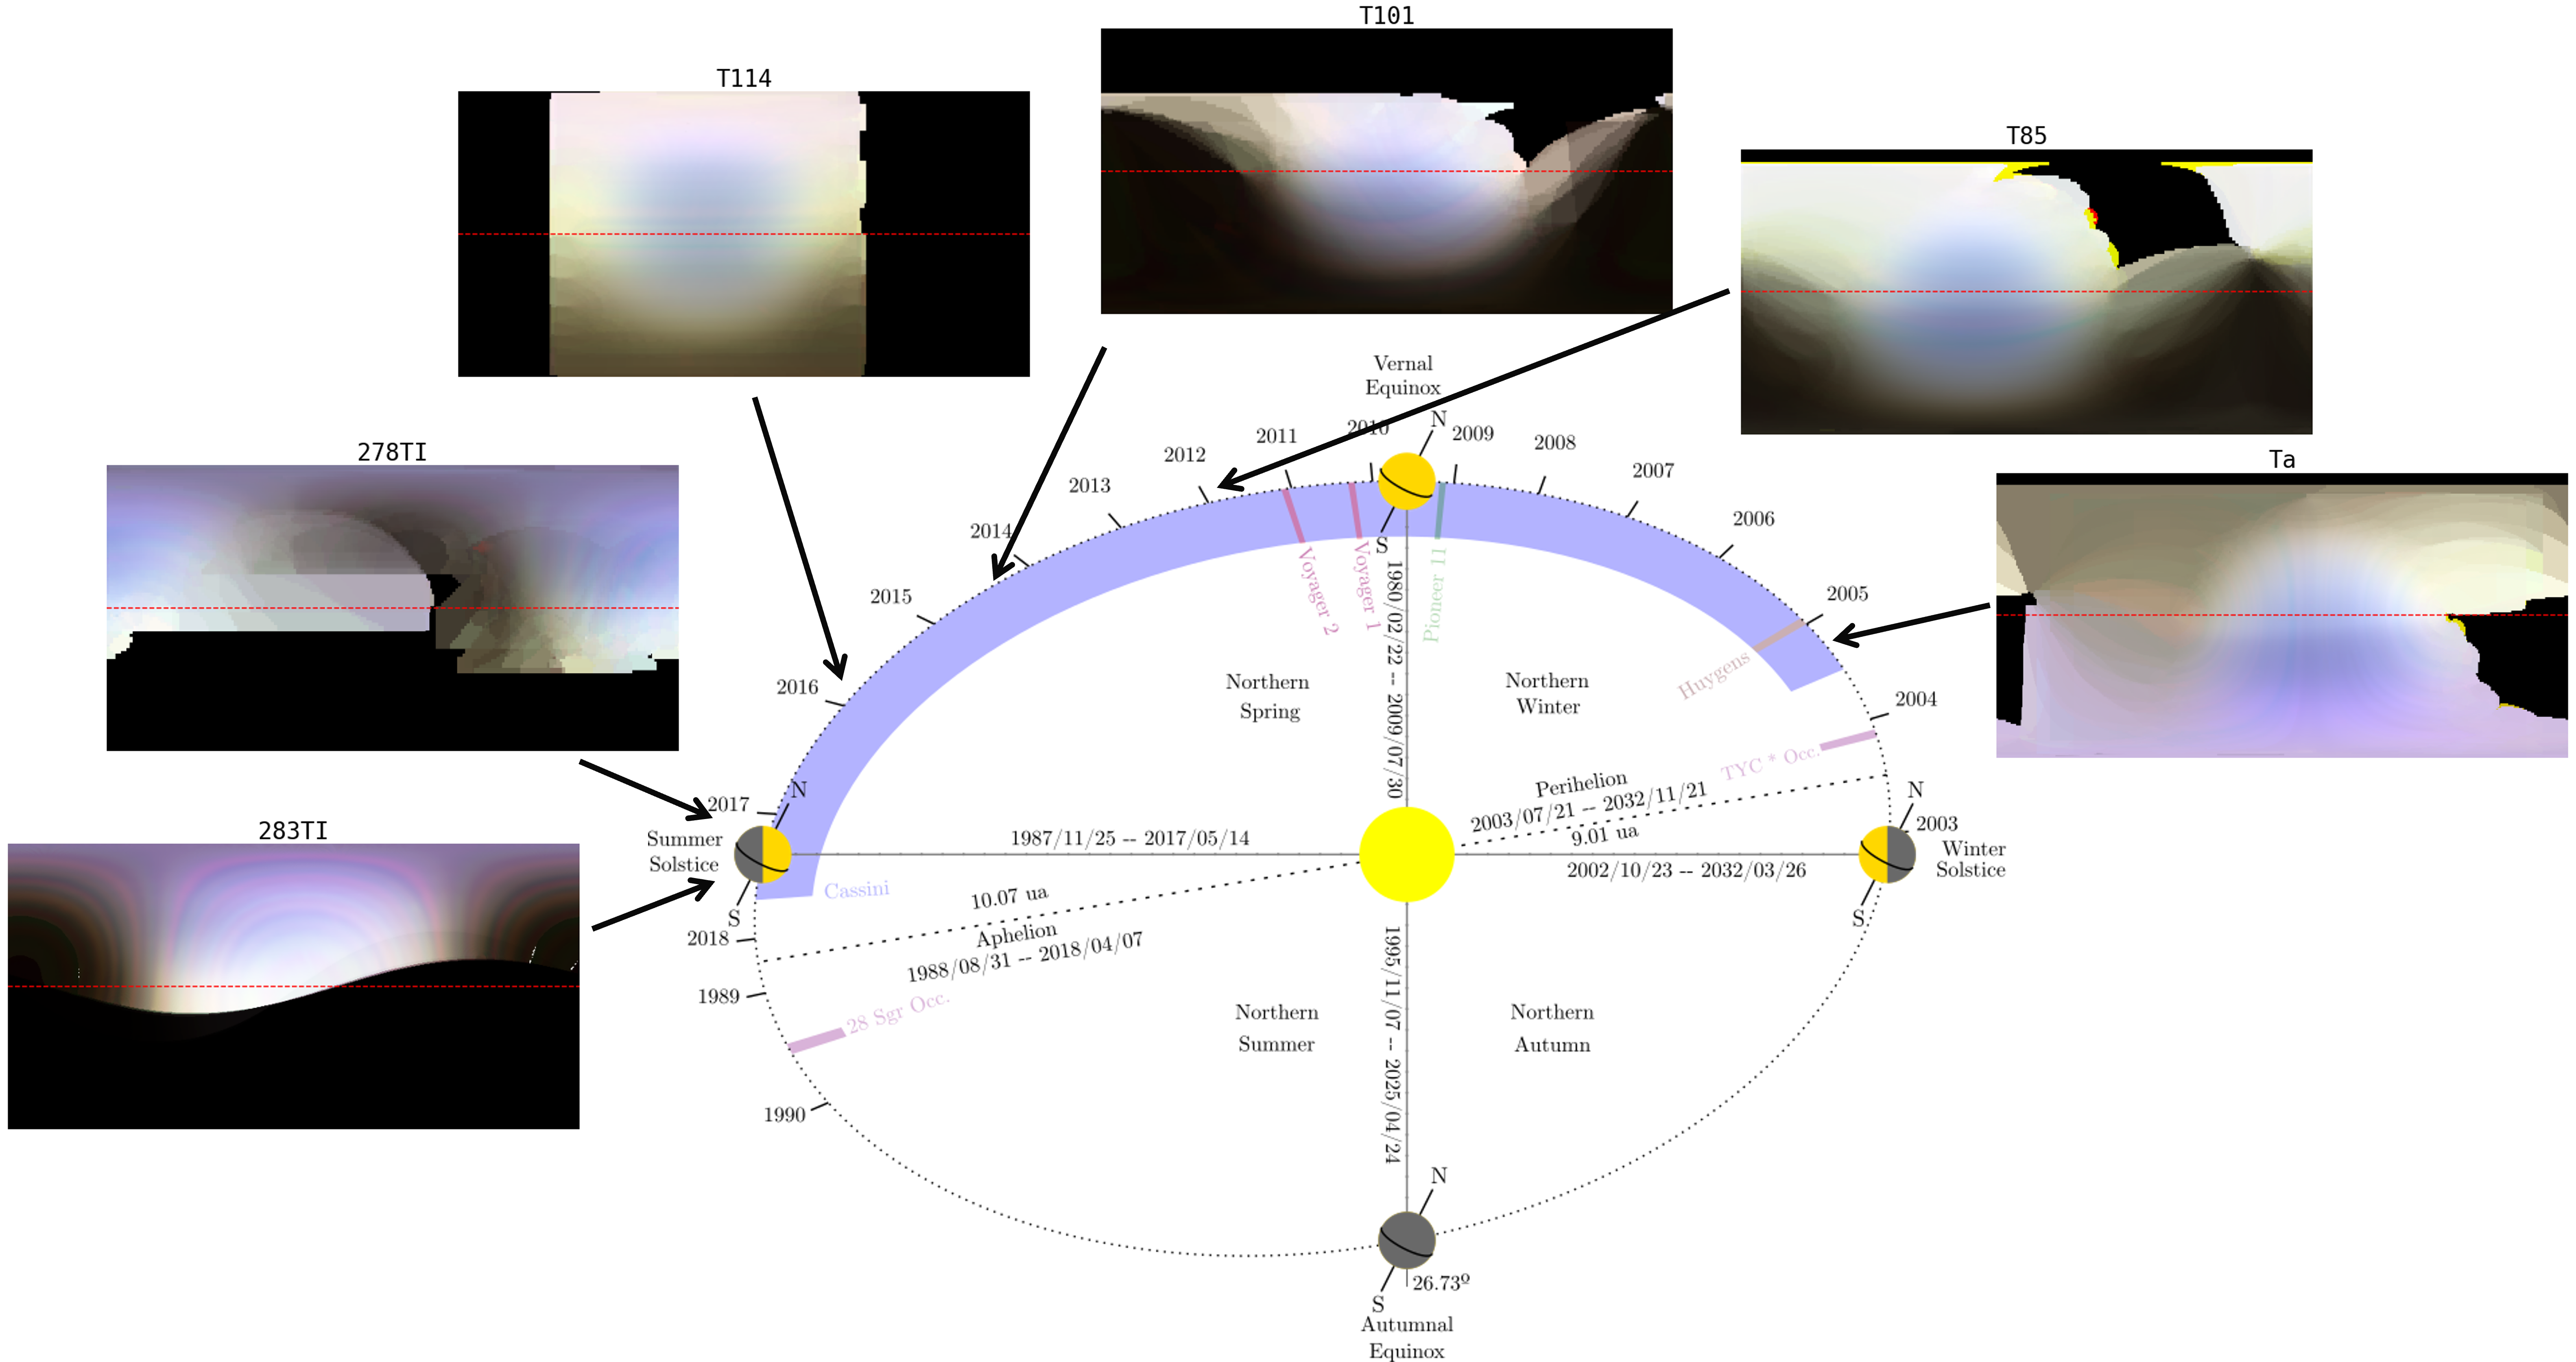
\includegraphics[width=\textwidth]{figures/new_timeline2.png}
\caption{\footnotesize A sequence of false-color (RGB: 0.725, 0.886, 1.003 $\mu$m), near-infrared VIMS cube images show the fading and flipping of the NSA boundary over a Titan half-year. The orbital diagram is adapted from Figure 1 of \citep{seignovert2021haze} to provide context with the Titan seasons. The red dashed lines indicate the equator. The Ta image has a sharp brightness contrast between the bright (violet) and dark (indigo) hemispheres. The NSA contrast was reduced, but the NSA boundary line was still visible below the equator by 2012 (T85). The NSA boundary line is lost in the T101 image, but some purple color remains. The lack of the NSA persists in the T114 image with a uniform (white) disk brightness profile. The NSA does not return until the near-end of the \textit{Cassini} mission in mid-2017 in the 278TI and 283TI images. The bright and dark hemispheres have flipped with the subtle boundary line above the equator.
\label{figure:nsadisappears}}
\end{figure*}

\begin{figure*}[tbhp]
\centering
\includegraphics[width=\textwidth]{figures/nsa_lat_timeline.png}
\caption{\footnotesize The timeline of the NSA boundary latitude as measured by instruments aboard Titan flyby missions and space telescopes. Before 2000, there was more uncertainty in the NSA boundary due to the reliance on noisier Hubble images. The period of rapid change applies to the early Hubble observations of seasonal NSA changes reported in \cite{lorenz2001titan}. A large segment of the 16-year seasonal cycle is precisely documented with the new VIMS NSA boundary data set. A period of a stable NSA from 2004 to 2014 was halted by an abrupt change in the fading of the NSA boundary from 2014 until its reversal and reappearance in 2017. 
Note that small systemic variations within the uncertainties exist in the NSA boundary latitude estimations between \textit{Cassini} ISS and VIMS images from 2004-2007. $L_s$ refers to solar longitude: 0\degree{} at Titan's Northern Spring Equinox.
\label{figure:nsaTime}}
\end{figure*}



\begin{deluxetable*}{|ccccccccc|}%rlcrrrrrr|}
\tablecaption{North-South Boundary Observations\label{table:data}}
%\rotate
\tablewidth{0pt}
\tablehead{
\colhead{} &
\colhead{} &
\colhead{} &
\colhead{Cassini} &
\colhead{} &
\colhead{} &
\colhead{Subsolar} &
\colhead{Boundary} &
\colhead{} \\
\colhead{Year} &
\colhead{Month} &
\colhead{Source} &
\colhead{flyby} &
\colhead{$\lambda$ ($\mu$m)} &
\colhead{$L_s$ ($^\circ$)} &
\colhead{Latitude ($^\circ$)} &
\colhead{Latitude ($^\circ$)} &
\colhead{Citation}
}\startdata
\hline
1980 & Nov & Voyager    &   & 0.450 &8 & 4   & $-5.5\pm 1$ & \citet{squyres1984voyager} \\
1981 & Aug & Voyager    &   & 0.450 &16 & 8   & $-5.5\pm 1$ & \citet{squyres1984voyager} \\
1990 & Aug & HST/WFPC   &   & 0.440 &122&23   & $32\pm 10$ & \citet{caldwell1992titan} \\
1992 & Aug & HST/WFPC   &  & 0.440 & 145&16   & $20\pm 10$ & \citet{smith1992titan} \\
1994 & Oct & HST/WFPC2  &   & 0.440 &168&5.8  & $15 \pm 5 $ & \citet{lorenz1997titan} \\
1995 & Aug & HST/WFPC2  &   & 0.440 &177&1.3  & $15 \pm 5 $ & \citet{lorenz1997titan} \\
1997 & Nov & HST/WFPC2  & &  0.889 & 202&-10.7& $10 \pm 15$ & \citet{lorenz1999seasonal}\\
2000 & Nov-Dec & HST/WFPC2  & &  889 & 242&-24  &   -- & \citet{lorenz2001titan} \\ 
2002 & Dec & HST/ACS    & & 0.435, 889&271&-26.7& $-20\pm 10$ & Inspection of \citet{lorenz2006seasonal} \\
2003 & Dec & HST/ACS    &  & 0.435 &  288&-25.6& $-20\pm 5$  & Inspection of \citet{lorenz2006seasonal} \\
2004 & Oct &Cassini/VIMS&   Ta &0.356-1.046 & 300&-23.2& $-12\pm3$& this work \\
2004 &Oct-Dec&Cassini/ISS& & 0.889 & 300&-23  & $-8\pm2$  & \citet{Roman2009}  \\
2005 &Feb-Dec&Cassini/ISS& & 0.889 & 309&-21  & $-8\pm2$    & \citet{Roman2009}  \\
2005 & Oct &Cassini/VIMS&   T8 & 0.356-1.046 &314&-19.6& $-12\pm3$& this work \\
2007 &May-Dec&Cassini/ISS& & 889 & 0.335&-11.5& $-8\pm2$    & \citet{Roman2009}  \\
2007 & May &Cassini/VIMS&  T31 & 0.356-1.046 & 333&-12.0&  $-12\pm3$& this work \\
2009 & Aug &Cassini/VIMS&   T61& 0.356-1.046 &  1&0.4 & $-12\pm3$& this work \\
2009 & Oct &Cassini/VIMS&   T62 &0.356-1.046 &   3&1 & $-12\pm3$& this work \\
2010 & Apr &Cassini/VIMS&  T67& 0.356-1.046 & 8& 8 & $-12\pm3$& this work \\
2011 & Dec &Cassini/VIMS&  T79& 0.356-1.046 & 29& 13 & $-10\pm4$& this work \\
2012 & Jul &Cassini/VIMS&  T85& 0.356-1.046 & 36& 15& $-10\pm4$& this work \\
2013 & Oct &Cassini/VIMS&  T92& 0.356-1.046 & 47& 19 & $-5\pm4$& this work \\
2014 & May &Cassini/VIMS&  T101& 0.356-1.046 & 57& 22& --& this work \\
2015 & Jan &Cassini/VIMS&  T108& 0.356-1.046 & 64& 24& --& this work \\
2015 & Nov &Cassini/VIMS&  T114& 0.356-1.046 & 74& 26 & --& this work \\
2017 & Jun &Cassini/VIMS&  278TI$^{1}$& 0.356-1.046 & 91& 27 & $10\pm3$& this work \\
2017 & July &Cassini/VIMS&  283TI$^{1}$& 0.356-1.046 & 92& 27& $10\pm4$& this work \\
\hline
\enddata
\tablenotetext{1}{non-targeted flyby of Titan}
%\tablecomments{. }
\end{deluxetable*}


\section{Conclusion}

The North-South Asymmetry in the haze between Titan's hemispheres tracks the evolution of haze abundances driven by the global atmospheric circulation of Titan. Given the \textit{Cassini} VIMS data, we can accurately monitor changes in the stratosphere of Titan through an entire half-year seasonal cycle using consistent instruments and analysis. 
We find the seasonal changes in the NSA boundary latitude and hemispheric flux dichotomy follow a two-step sequence. A period of constant NSA boundary latitude with a slow changing flux ratio for several years from the start of northern winter in 2004 until a few years after the vernal equinox in 2011. 
In 2012, a rapid change in the NSA boundary shifted towards the equator and subsequently fades away until reappearing in the opposite hemisphere during northern summer in 2017. %do not correspond with changes in the orbital eccentricity of Saturn%, with a 14-year cycle as opposed to the 16-year cycle. 
The current study also finds a detectable few-degree tilt of the NSA that reinforces the presence of a super-rotating atmosphere. We demonstrate that the NSA boundary is detectable at higher phase angles up to 90\degree{} with reducing I/F contrast.

In the not-too-distant future, missions such as the Dragonfly drone or an orbiter \citep{lorenz2018dragonfly, barnes2021science} could lead to an active probe that can measure in-situ changes in the lower atmosphere on a more localized level instead of through changes in haze observed from orbit. Future analysis can examine the long-term effects of a super-rotating atmosphere on Titan, and data taken over a larger period of time can aim to gain a better understanding of the movement of the atmosphere relative to the rotational axis. In addition, a study analyzing the correlation between the polar hood and the seasonal motion of the NSA boundary could reveal new details about the haze distributions. 

\acknowledgements

The authors acknowledge support from the NASA/ESA \emph{Cassini} project.

\bibliography{NSAreferences.bib}
\bibliographystyle{aasjournal}%icarus}


\end{document}
